\newpage
\maketitle
\begin{center}
\Large \textbf{第1章 强化学习概述} \quad 
\end{center}
\begin{abstract}
在本章中我们将讨论强化学习中的环境、Agent、状态、Action和奖励,并重点讨论MDP相关内容。
\end{abstract}
\section{MDP概述}
一个典型的强化学习系统结构如下所示:
\begin{figure}[H]
	\caption{典型强化学习系统架构图}
	\label{p000001}
	\centering
	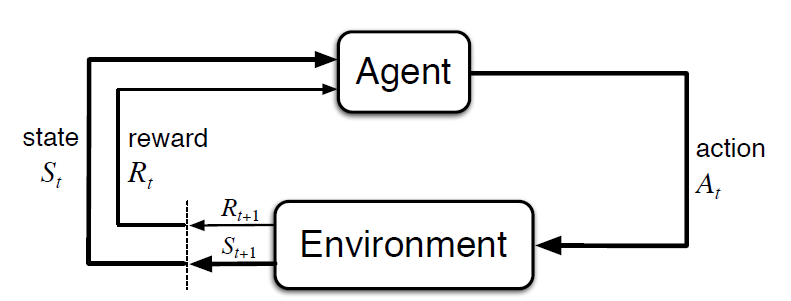
\includegraphics[width=15cm]{images/p000001}
\end{figure}
如图所示:
\begin{enumerate}
    \item 在$t$时刻Agent观察到环境状态$S_{t}$,并得到上一时刻所采取的行动$A_{t-1}$(在图中未画出)所得到的
奖励$r_{t}$;
    \item Agent根据环境状态$S_{t}$,根据某种策略$\pi$,选择行动$A_{t}$;
    \item 环境接收到Agent的行动$A_{t}$后,根据环境的动态特性,转移到新的状态$S_{t+1}$,并产生$R_{t}$的奖励
信号;
\end{enumerate}
\subsection{典型环境}
\subsubsection{Bandit Walk环境}
下面我们来研究一个最简单的强化学习环境,叫Bandit Walk,如下所示:
\begin{figure}[H]
	\caption{Bandit Walk环境图}
	\label{p000002}
	\centering
	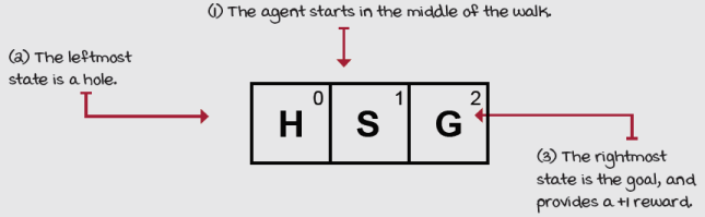
\includegraphics[width=15cm]{images/p000002}
\end{figure}
如图所示,Agent初始时位于中间的S格,状态编号为$S_{0}$,其可以采取向左、向右两个动作,向左则进入状态$H$,其是一个洞,就会掉到洞里,
过程就会结束,此时得到的奖励为0;当Agent采取向右行动时,就会进入G状态,此时会获得奖励+1,由此可见其是一个确定性的环境,就是说当
Agent采取向右行动时,会100\%确定进行G状态。我们可以通过如下的图来表示上述过程:
\begin{figure}[H]
	\caption{Bandit Walk环境MDP图}
	\label{p000003}
	\centering
	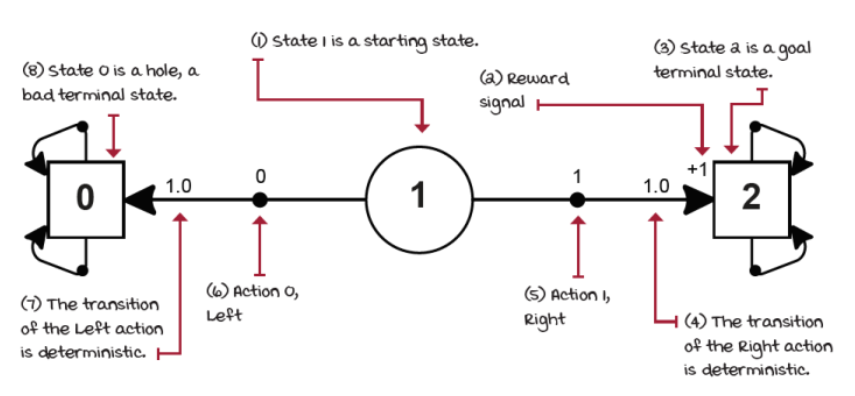
\includegraphics[width=15cm]{images/p000003}
\end{figure}
如图所示:
\begin{itemize}
    \item 在初始状态$S_{0}$时,有两个可选行动,分别表示为向左、向右的直线;
    \item 当采取向右行动时,就会到达小黑点位置,然后由环境决定将转到哪个状态,以及转到这个状态的概率,以本例为例,其就是以100\%
的概率转到G状态$S_{2}$,其中小黑点上面的1代表行动编号,向右简头上面的1.0代表100\%的概率,向右简头处的1代表奖励为+1;
\end{itemize}
我们首先安装所需要的库:
\lstset{language=PYTHON, caption={安装gmy库}, label={pip-install-gym}}
\begin{lstlisting}
pip install gym -i https://pypi.tuna.tsinghua.edu.cn/simple 
\end{lstlisting}
下面我们用Python对象来表示这一过程:
\lstset{language=PYTHON, caption={Bandit Walk python程序}, label={bandit-walk-python-env}}
\begin{lstlisting}
P = {
    0: {
        0: [(1.0, 0, 0.0, True)],
        1: [(1.0, 0, 0.0, True)]
    },
    1: {
        0: [(1.0, 0, 0.0, True)],
        1: [(1.0, 2, 1.0, True)]
    },
    2: {
        0: [(1.0, 2, 0.0, True)],
        1: [(1.0, 2, 0.0, True)]
    }
}
print(P)
\end{lstlisting}
代码解读如下所示:
\begin{itemize}
    \item P为一个字典对象,其键值0、1、2代表三个状态;
    \item P的键值0:其同样是一个字典对象,键值代表可以采取的行动,0代表向右,1代表向右;
    \item P的键值0下键值0:即在状态0下面采取行动0,其值为一个数组,代表由环境决定要转到哪个状态,转到每个状态为一个Turple,含
义为:(概率, 目的状态,获得奖励,新状态是否为终止状态),注意:我们规定在终止状态采取任何行动都会回到自身;
\end{itemize}
上面我们仅举了一个例子,其他状态读者可以自己解析出来。
\subsubsection{Bandit Slippery Walk环境}
在上面的环境中,我们向左移动,环境会确定地向左移动。但是在本节中,当我们向左移动时,环境在80\%的情况下会向左移动,20\%的情况会
向右移动。如下图所示:
\begin{figure}[H]
	\caption{Bandit Slippery Walk环境图}
	\label{p000004}
	\centering
	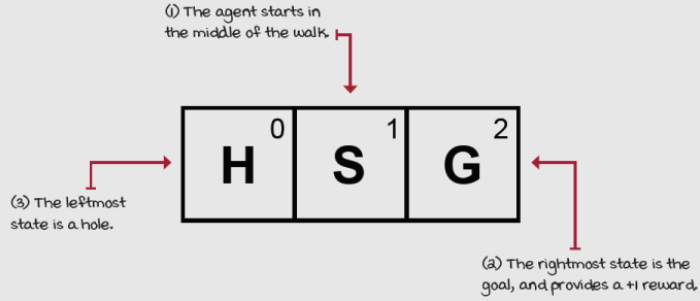
\includegraphics[width=15cm]{images/p000004}
\end{figure}
除了环境的随机性之外,环境